\documentclass[aspectratio=1610, polish]{beamer}
\usepackage{babel}
\usepackage{polski}
\usepackage[utf8]{inputenc}
\usepackage{graphicx}
\graphicspath{{../figures/}}
\usepackage{booktabs}
\usepackage{tabularx}
\usepackage{array}
\usepackage{colortbl}
\usepackage{xcolor}
\usepackage{amsmath}
\usepackage{amssymb}
\usepackage{tikz}
\usetikzlibrary{positioning, calc, arrows.meta, shapes.geometric}

\mode<beamer>{
    \hypersetup{pdfpagemode=FullScreen}
    \usetheme[parttitle=rightfooter]{AGH}
}

% Pastelowa paleta zgodna z głównym raportem (Obsidian-friendly)
\definecolor{obsBlueBg}{HTML}{DDE9F4}    \definecolor{obsBlueFg}{HTML}{2E5C8A}
\definecolor{obsGreenBg}{HTML}{D9EAD3}   \definecolor{obsGreenFg}{HTML}{38761D}
\definecolor{obsAmberBg}{HTML}{F4E3C3}   \definecolor{obsAmberFg}{HTML}{B45F06}
\definecolor{obsPurpleBg}{HTML}{E4D6EF}  \definecolor{obsPurpleFg}{HTML}{6A3D9A}
\definecolor{obsRedBg}{HTML}{F4CCCC}     \definecolor{obsRedFg}{HTML}{990000}
\definecolor{obsOrangeBg}{HTML}{FCE5CD}  \definecolor{obsOrangeFg}{HTML}{B45F06}

\definecolor{ok}{RGB}{220,237,200}
\definecolor{warning}{RGB}{255,243,205}
\definecolor{danger}{RGB}{255,220,220}

\author[Piotrowski, Przeździk]{Dawid Piotrowski \and Julia Przeździk}
\date{29 kwietnia 2026}
\title{Równoległy algorytm genetyczny}
\subtitle{do układania planu zajęć uniwersyteckich --- Projekt nr 26}
\institute[AGH]{
    Wydział Fizyki i Informatyki Stosowanej\\
    Akademia Górniczo-Hutnicza w Krakowie\\[2pt]
    \small Systemy Równoległe i Rozproszone --- Lab.~9, gr.~1 \\
    \scriptsize prowadzący: dr inż. Piotr Gronek
}

\begin{document}
\maketitle

%%%%%%%%%%%%%%%%%%%%%%%%%%%%%%%%%%%%%%%%%%%%%%%%%%%%%%%%%%%%%%%%%%%%%
\begin{frame}{Plan prezentacji}
    \tableofcontents
\end{frame}

%%%%%%%%%%%%%%%%%%%%%%%%%%%%%%%%%%%%%%%%%%%%%%%%%%%%%%%%%%%%%%%%%%%%%
\section{Problem i skala}
%%%%%%%%%%%%%%%%%%%%%%%%%%%%%%%%%%%%%%%%%%%%%%%%%%%%%%%%%%%%%%%%%%%%%

\begin{frame}{University Course Timetabling Problem}
\textbf{Cel:} przypisać zdarzenia (wykłady, laboratoria, seminaria) do par
\((\text{slot czasowy}, \text{sala})\), spełniając ograniczenia twarde
i minimalizując karę za miękkie.

\vspace{0.6em}
\begin{columns}[T]
\column{0.5\textwidth}
\textbf{Ograniczenia twarde (kary $\times$1000):}
\begin{itemize}\small
    \item kolizja sali
    \item kolizja prowadzącego
    \item kolizja grupy studenckiej
    \item niewłaściwy typ sali (lab/wykład)
    \item przepełnienie dnia
\end{itemize}

\column{0.5\textwidth}
\textbf{Ograniczenia miękkie (kary $\times$1--2):}
\begin{itemize}\small
    \item okienka w planie grupy
    \item kompaktowość dni
    \item zajęcia późnym popołudniem
    \item kompaktowość prowadzących
    \item pojemność sal vs liczność grup
    \item ciągłość budynków (D-7 / D-10 / D-11)
\end{itemize}
\end{columns}

\vspace{0.7em}
\begin{center}
\fcolorbox{black}{ok}{\parbox{0.85\textwidth}{\centering
\textbf{Realny dataset (UniTime AGH, sem. letni 2026):}
\textbf{633} zdarzeń, \textbf{41} sal, \textbf{161} prowadzących, \textbf{191} grup,
\textbf{35} slotów (5 dni $\times$ 7 bloków 1.5\,h)
}}
\end{center}
\end{frame}

%%%%%%%%%%%%%%%%%%%%%%%%%%%%%%%%%%%%%%%%%%%%%%%%%%%%%%%%%%%%%%%%%%%%%
\section{Algorytm genetyczny}
%%%%%%%%%%%%%%%%%%%%%%%%%%%%%%%%%%%%%%%%%%%%%%%%%%%%%%%%%%%%%%%%%%%%%

\begin{frame}{Kodowanie i fitness}
\textbf{Chromosom} = wektor genów, gen \(g_i = (\text{slot}_i, \text{sala}_i)\)
dla każdego zdarzenia. Długość chromosomu = liczba zdarzeń.

\vspace{0.5em}
\textbf{Fitness dwupoziomowy:}
\[
\mathrm{fitness}(c) = 1000 \cdot H(c) + S(c)
\]
\begin{itemize}\small
    \item \(H(c)\) --- liczba naruszeń twardych (do wyzerowania)
    \item \(S(c)\) --- suma kar miękkich (do minimalizacji po osiągnięciu \(H=0\))
\end{itemize}

\vspace{0.4em}
Porównywanie osobników: dwupoziomowo \((H, S)\) leksykograficznie ---
osobnik z \(H=0\) zawsze lepszy od dowolnego z \(H>0\).
\end{frame}

\begin{frame}{Operatory genetyczne}
\renewcommand{\arraystretch}{1.15}
\centering\small
\begin{tabular}{>{\bfseries}l p{0.62\textwidth}}
\toprule
Selekcja      & turniej $K=3$, dwupoziomowe porównanie \((H, S)\) \\
Krzyżowanie   & uniform 50/50, prawdopodobieństwo $p_c = 0{,}8$ \\
Mutacja       & adaptacyjna: $5\%$ przy $H>0$, $1\%$ przy $H=0$ \\
Naprawa       & zachłanna: 20 losowych prób + systematyczny skan \\
Elityzm       & najlepszy osobnik zawsze przechodzi do następnego pokolenia \\
Local search  & hill climbing 5000 iteracji po zakończeniu GA \\
\bottomrule
\end{tabular}

\vspace{0.7em}
\begin{center}
\fcolorbox{black}{ok}{\parbox{0.85\textwidth}{\centering\small
\textbf{Terminacja:} stagnacja $\geq 200$ pokoleń \emph{lub}
$\mathrm{fitness}=0$ \emph{lub} max 500 pokoleń.\\
Synchroniczna terminacja na klastrze przez \texttt{MPI\_Allreduce(MAX)}.
}}
\end{center}
\end{frame}

%%%%%%%%%%%%%%%%%%%%%%%%%%%%%%%%%%%%%%%%%%%%%%%%%%%%%%%%%%%%%%%%%%%%%
\section{Architektura równoległa}
%%%%%%%%%%%%%%%%%%%%%%%%%%%%%%%%%%%%%%%%%%%%%%%%%%%%%%%%%%%%%%%%%%%%%

\begin{frame}{Island Model --- topologia pierścienia}
\centering
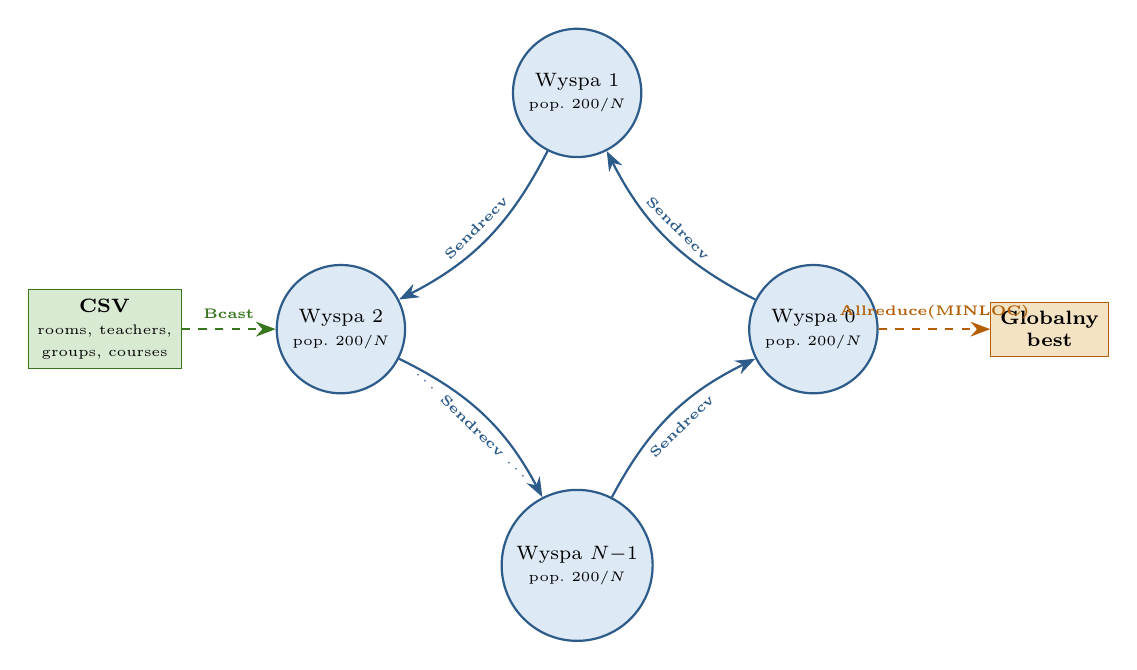
\begin{tikzpicture}[
    isl/.style={draw, circle, minimum size=1.6cm, align=center, font=\scriptsize, thick},
    arr/.style={-{Stealth[length=2.5mm]}, thick, obsBlueFg},
    darr/.style={-{Stealth[length=2.5mm]}, thick, dashed, obsRedFg},
    barr/.style={-{Stealth[length=2.5mm]}, thick, obsGreenFg, dashed},
]
\node[isl, fill=obsBlueBg, draw=obsBlueFg] (r0) at (0:3)    {Wyspa 0\\\tiny pop.~200/$N$};
\node[isl, fill=obsBlueBg, draw=obsBlueFg] (r1) at (90:3)   {Wyspa 1\\\tiny pop.~200/$N$};
\node[isl, fill=obsBlueBg, draw=obsBlueFg] (r2) at (180:3)  {Wyspa 2\\\tiny pop.~200/$N$};
\node[isl, fill=obsBlueBg, draw=obsBlueFg] (r3) at (270:3)  {Wyspa $N{-}1$\\\tiny pop.~200/$N$};

\draw[arr] (r0) to[bend left=18] node[midway, sloped, above, font=\tiny\bfseries] {Sendrecv} (r1);
\draw[arr] (r1) to[bend left=18] node[midway, sloped, above, font=\tiny\bfseries] {Sendrecv} (r2);
\draw[arr] (r2) to[bend left=18] node[midway, sloped, below, font=\tiny\bfseries] {$\cdots$ Sendrecv $\cdots$} (r3);
\draw[arr] (r3) to[bend left=18] node[midway, sloped, below, font=\tiny\bfseries] {Sendrecv} (r0);

\node[draw, rectangle, fill=obsGreenBg, draw=obsGreenFg, font=\scriptsize, align=center]
    (csv) at (-6, 0) {\textbf{CSV}\\\tiny rooms, teachers,\\\tiny groups, courses};
\draw[barr] (csv) -- node[midway, above, font=\tiny\bfseries] {Bcast} (r2);

\node[draw, rectangle, fill=obsAmberBg, draw=obsAmberFg, font=\scriptsize, align=center]
    (best) at (6, 0) {\textbf{Globalny}\\\textbf{best}};
\draw[darr, obsAmberFg] (r0) -- node[midway, above, font=\tiny\bfseries] {Allreduce(MINLOC)} (best);
\end{tikzpicture}

\vspace{0.4em}
\begin{center}
\fcolorbox{black}{ok}{\parbox{0.7\textwidth}{\centering\scriptsize
Każda wyspa ewoluuje niezależną subpopulację. Migracja pierścieniowa co 50 pokoleń ---
najlepszy osobnik wymieniany z sąsiadem.
}}
\end{center}
\end{frame}

\begin{frame}{Operacje MPI używane w projekcie}
\centering\small
\renewcommand{\arraystretch}{1.25}
\begin{tabular}{>{\tt}l p{0.5\textwidth} l}
\toprule
\textbf{Prymityw} & \textbf{Zastosowanie} & \textbf{Częstotliwość} \\
\midrule
MPI\_Bcast              & dystrybucja \texttt{ProblemData} z rank~0 & raz, na starcie \\
MPI\_Sendrecv           & migracja w pierścieniu (best $\to$ sąsiad) & co 50 pokoleń \\
MPI\_Allreduce(MINLOC)  & wybór globalnego best & na końcu \\
MPI\_Allreduce(MAX)     & synchronizacja terminacji (stop flag) & co pokolenie \\
MPI\_Wtime              & pomiar czasu (speedup) & przed/po pętli GA \\
\bottomrule
\end{tabular}

\vspace{0.7em}
\begin{itemize}\small
    \item Niezależne strumienie PRNG (PCG32, \texttt{initseq=rank}) --- nieskorelowane subpopulacje
    \item Serializacja chromosomu do flat buffer \texttt{int[]} przed migracją
\end{itemize}
\end{frame}

%%%%%%%%%%%%%%%%%%%%%%%%%%%%%%%%%%%%%%%%%%%%%%%%%%%%%%%%%%%%%%%%%%%%%
\section{Implementacja}
%%%%%%%%%%%%%%%%%%%%%%%%%%%%%%%%%%%%%%%%%%%%%%%%%%%%%%%%%%%%%%%%%%%%%

\begin{frame}{Stack i klaster}
\begin{columns}[T]
\column{0.5\textwidth}
\textbf{Stack technologiczny:}
\begin{itemize}\small
    \item \textbf{C99} (wymaganie prowadzącego)
    \item \textbf{MPICH 5.0} + CUDA 12.1 (runtime klaster)
    \item \textbf{PCG32} --- per-rank PRNG
    \item \textbf{gnuplot} --- wykresy speedup/konwergencji
    \item \textbf{Make} --- 7 reguł (\texttt{run}, \texttt{benchmark}, \texttt{plot}, \texttt{archive}, \ldots)
\end{itemize}

\column{0.5\textwidth}
\textbf{Klaster AGH (sala 204, D-10):}
\begin{itemize}\small
    \item \texttt{taurus.fis.agh.edu.pl} --- node logujący
    \item 16 węzłów \texttt{stud204-01..16}
    \item kompilacja: \texttt{-Wl,--allow-shlib-undefined}\\(taurus bez sterownika NVIDIA)
    \item uruchamianie: \texttt{mpiexec -f nodes -n N ./timetable\_ga}
\end{itemize}
\end{columns}

\vspace{0.7em}
\centering
\fcolorbox{black}{ok}{\parbox{0.85\textwidth}{\centering\small
\textbf{6 plików C} ($\sim$2,300 LoC): \texttt{main.c}, \texttt{ga.c/h}, \texttt{fitness.c/h},
\texttt{io.c/h}, \texttt{types.h}, \texttt{pcg\_basic.c/h}
}}
\end{frame}

%%%%%%%%%%%%%%%%%%%%%%%%%%%%%%%%%%%%%%%%%%%%%%%%%%%%%%%%%%%%%%%%%%%%%
\section{Wyniki}
%%%%%%%%%%%%%%%%%%%%%%%%%%%%%%%%%%%%%%%%%%%%%%%%%%%%%%%%%%%%%%%%%%%%%

\begin{frame}{Przyspieszenie na klastrze AGH (5 runów / konfigurację)}
\centering\small
\renewcommand{\arraystretch}{1.2}
\begin{tabular}{rrrrrr}
\toprule
\textbf{Zdarzenia} & \textbf{$T_1$ [s]} & \textbf{$T_4$ [s]} & \textbf{$T_8$ [s]} & \textbf{$T_{16}$ [s]} & \textbf{$S_{16}$} \\
\midrule
100              & 3.20    & 0.79  & 0.44  & 0.27 & \cellcolor{ok}\textbf{11.96$\times$} \\
200              & 15.03   & 2.38  & 1.11  & 0.61 & \cellcolor{ok}\textbf{24.55$\times$} $\uparrow$ \\
400              & 53.44   & 10.38 & 4.60  & 1.86 & \cellcolor{ok}\textbf{28.73$\times$} $\uparrow$ \\
1058 (UniTime)   & 189.94  & 49.34 & 23.57 & 9.70 & \cellcolor{ok}\textbf{19.59$\times$} \\
\bottomrule
\end{tabular}

\vspace{0.7em}
\begin{itemize}\small
    \item \textbf{0 naruszeń twardych} we wszystkich konfiguracjach $\to$ feasible plan zawsze
    \item \textbf{Super-liniowy speedup} ($S_{16}>16\times$) dla 200 i 400 zdarzeń ---
          efekt wielowyspowej eksploracji + wymiany dobrych cech przez migrację
    \item Naruszenia miękkie też niższe równolegle: 400~zdarzeń: 675 $\to$ 645 (1$\to$16~proc.)
\end{itemize}
\end{frame}

\begin{frame}{Wykres przyspieszenia}
\centering
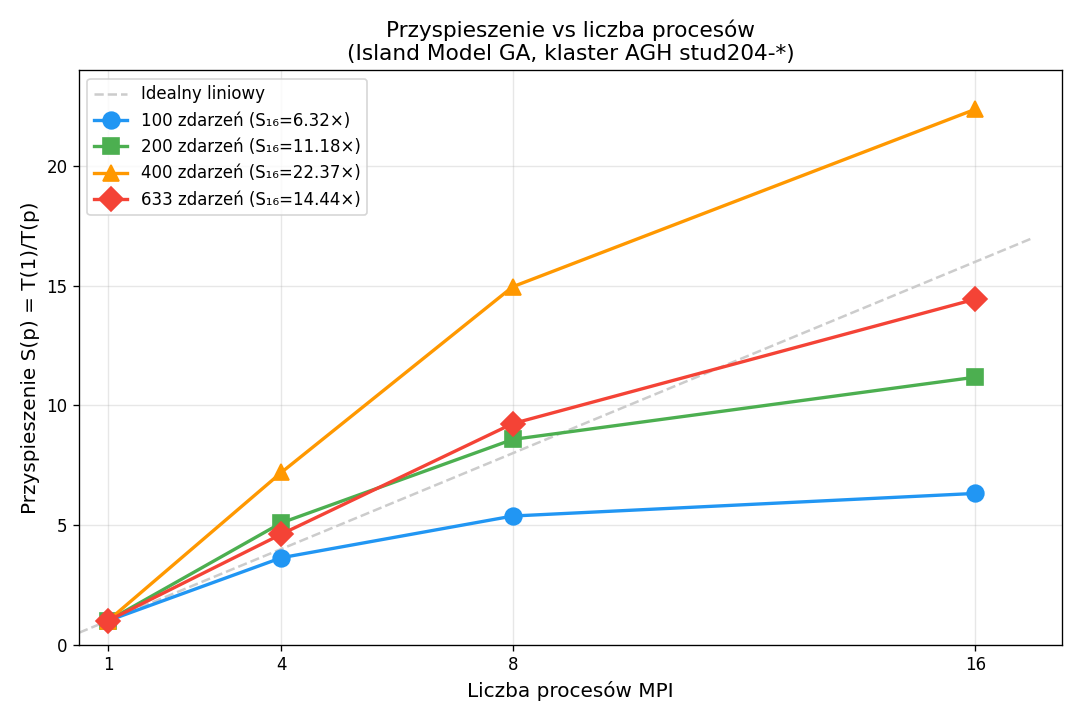
\includegraphics[height=0.78\textheight]{speedup.png}
\end{frame}

\begin{frame}{Konwergencja per wyspa --- 16 wysp, 1058 zdarzeń}
\centering
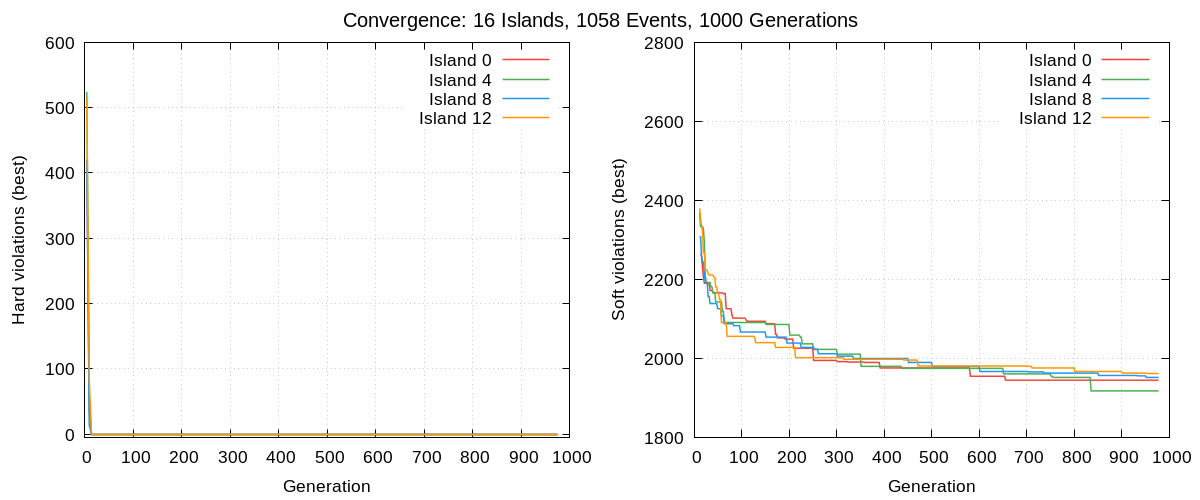
\includegraphics[height=0.78\textheight]{convergence.png}
\end{frame}

%%%%%%%%%%%%%%%%%%%%%%%%%%%%%%%%%%%%%%%%%%%%%%%%%%%%%%%%%%%%%%%%%%%%%
\section{Wnioski}
%%%%%%%%%%%%%%%%%%%%%%%%%%%%%%%%%%%%%%%%%%%%%%%%%%%%%%%%%%%%%%%%%%%%%

\begin{frame}{Podsumowanie projektu}
\textbf{Zrealizowane:}
\begin{itemize}\small
    \item Pełny GA: dwupoziomowy fitness, naprawa zachłanna, local search
    \item Island Model + ring migration + Allreduce + niezależne PCG32
    \item Realny dataset UniTime AGH (633 zdarzeń) + 3 podzbiory skalowalności
    \item Realne benchmarki na 16-węzłowym klastrze --- super-liniowy speedup
\end{itemize}

\vspace{0.4em}
\textbf{Wnioski techniczne:}
\begin{itemize}\small
    \item Island Model dobrze skaluje się do $N=16$, narzut komunikacji
          rośnie z chromosomem ($\sim$8.3 KB na migrację dla 1058 zdarzeń)
    \item Naruszenia miękkie spadają z liczbą wysp dzięki bogatszej eksploracji
    \item Synchroniczna terminacja przez Allreduce(MAX) eliminuje deadlocki
          przy wczesnej zbieżności jednej wyspy
\end{itemize}

\vspace{0.4em}
\begin{center}
\fcolorbox{black}{ok}{\parbox{0.85\textwidth}{\centering\small
\textbf{Repo:} \url{https://github.com/LeoTheOriginal/parallel-ga-timetabling}\\
\textbf{Raport:} \url{https://github.com/LeoTheOriginal/parallel-ga-timetabling-report}
}}
\end{center}
\end{frame}

%%%%%%%%%%%%%%%%%%%%%%%%%%%%%%%%%%%%%%%%%%%%%%%%%%%%%%%%%%%%%%%%%%%%%
\section{Demo i Q\&A}
%%%%%%%%%%%%%%%%%%%%%%%%%%%%%%%%%%%%%%%%%%%%%%%%%%%%%%%%%%%%%%%%%%%%%

\begin{frame}{Demo --- działanie na klastrze}
\centering\small
\textbf{Plan demo (taurus + stud204-NN):}
\begin{enumerate}
    \item \texttt{ssh 2piotrowski@taurus.fis.agh.edu.pl} + środowisko MPI
    \item \texttt{make} --- kompilacja
    \item \texttt{make run} --- 1~proces, dane przykładowe (\texttt{simple\_n100/})
    \item \texttt{mpiexec -f nodes -n 16 ./timetable\_ga data/simple\_n400/}
    \item Wynik: \texttt{schedule.csv} + \texttt{timetable.txt} + \texttt{convergence\_thread*.csv}
    \item Porównanie czasów $T_1$ vs $T_{16}$ na żywo
\end{enumerate}

\vspace{1em}
\begin{center}
\Large \textbf{Pytania?}

\vspace{0.5em}
\small Dziękujemy za uwagę.\\
\scriptsize Dawid Piotrowski \quad $\cdot$ \quad Julia Przeździk
\end{center}
\end{frame}

\end{document}
